\section{Ablation Study}
\label{sec:ablation}

An ablation removes or replaces one component and measures what changes. No new experiment
was run for this section: it gathers the component comparisons the project had already made,
on the pre-therapy session of the \rqTwoHTwoAN{} patients with the chronological split.
\textbf{P} marks a pre-registered comparison (confirmatory, or a descriptive reference or
exploratory study named in the plan). \textbf{X} marks one added after the confirmatory results
(post hoc): its settings were fixed in a file before its own test scores, but it was chosen
with the earlier results in view, and it is uncorrected for multiplicity. Each group in
Tables~\ref{tab:abl-model} and~\ref{tab:abl-use} names its results file under
\texttt{results/summary/}. Differences are paired, variant minus reference, in points with
95\,\% bootstrap CIs; a dash means no paired difference was computed.

\begin{table*}[!t]
  \centering
  \caption{Ablations of the decoder's inputs and model. Balanced accuracy (\%) on runs 3--4
  of the pre-therapy session, $n = \rqFourCueN$ patients; AH: affected hand; SF: sixth finger.
  Label P: pre-registered; X: exploratory, added after the confirmatory results.}
  \label{tab:abl-model}
  \footnotesize
  \setlength{\tabcolsep}{4pt}
  \renewcommand{\arraystretch}{1.1}
  \begin{tabularx}{\textwidth}{@{}L>{\raggedright\arraybackslash}p{1.95cm}>{\raggedright\arraybackslash}p{3.1cm}cc>{\raggedright\arraybackslash}p{2.75cm}c@{}}
    \toprule
    Variant & Task & Reference & Variant & Reference & Difference [95\,\% CI] & Label \\
    \midrule
    \multicolumn{7}{@{}l}{\emph{Channels: TS+LR on a subset of the 40 channels}} \\
    \multicolumn{7}{@{}l}{\quad(\src{rq4\_visual\_cue\_paired.csv})} \\
    14 central channels & SF vs rest & all 40 & \rqFourCueSfRestCentralMean & \rqFourCueSfRestAllChannelsMean & \rqFourCueSfRestCentralVsAllChannelsDiff{} [\rqFourCueSfRestCentralVsAllChannelsDiffCiLo, \rqFourCueSfRestCentralVsAllChannelsDiffCiHi] & X \\
    5 parieto-occipital channels & SF vs rest & all 40 & \rqFourCueSfRestParietoOccipitalMean & \rqFourCueSfRestAllChannelsMean & \rqFourCueSfRestParietoOccipitalVsAllChannelsDiff{} [\rqFourCueSfRestParietoOccipitalVsAllChannelsDiffCiLo, \rqFourCueSfRestParietoOccipitalVsAllChannelsDiffCiHi] & X \\
    14 central channels & AH vs SF & all 40 & \rqFourCueAhSfCentralMean & \rqFourCueAhSfAllChannelsMean & \rqFourCueAhSfCentralVsAllChannelsDiff{} [\rqFourCueAhSfCentralVsAllChannelsDiffCiLo, \rqFourCueAhSfCentralVsAllChannelsDiffCiHi] & X \\
    5 parieto-occipital channels & AH vs SF & all 40 & \rqFourCueAhSfParietoOccipitalMean & \rqFourCueAhSfAllChannelsMean & \rqFourCueAhSfParietoOccipitalVsAllChannelsDiff{} [\rqFourCueAhSfParietoOccipitalVsAllChannelsDiffCiLo, \rqFourCueAhSfParietoOccipitalVsAllChannelsDiffCiHi] & X \\
    \midrule
    \multicolumn{7}{@{}l}{\emph{Pre-training and fine-tuning of EEGNet}} \\
    \multicolumn{7}{@{}l}{\quad(\src{ex1\_transfer\_ah\_sf\_paired.csv}; last row \src{calib\_curves.csv})} \\
    Pre-trained and fine-tuned EEGNet & AH vs SF & the same, not fine-tuned & \exOneArmBVsArmBPretrainedArmMean & \exOneArmBVsArmBPretrainedBaseMean & \exOneArmBVsArmBPretrainedDiff{} [\exOneArmBVsArmBPretrainedDiffCiLo, \exOneArmBVsArmBPretrainedDiffCiHi] & X \\
    Pre-trained and fine-tuned EEGNet & AH vs SF & pre-trained, no target data & \exOneArmBVsZeroShotArmMean & \exOneArmBVsZeroShotBaseMean & \exOneArmBVsZeroShotDiff{} [\exOneArmBVsZeroShotDiffCiLo, \exOneArmBVsZeroShotDiffCiHi] & X \\
    Pre-trained and fine-tuned EEGNet & AH vs SF & EEGNet from scratch & \exOneArmBVsEegnetScratchArmMean & \exOneArmBVsEegnetScratchBaseMean & \exOneArmBVsEegnetScratchDiff{} [\exOneArmBVsEegnetScratchDiffCiLo, \exOneArmBVsEegnetScratchDiffCiHi] & X \\
    Pre-trained and fine-tuned EEGNet & AH vs SF & TS+LR & \exOneArmBVsTsLrArmMean & \exOneArmBVsTsLrBaseMean & \exOneArmBVsTsLrDiff{} [\exOneArmBVsTsLrDiffCiLo, \exOneArmBVsTsLrDiffCiHi] & X \\
    Pre-trained EEGNet, fine-tuned on all trials & 3 classes & the same, no fine-tuning ($k = 0$) & \rqTwoRestAhSfEegnetEaFtKAllMean & \rqTwoRestAhSfEegnetEaFtKZeroMean & -- & P \\
    \midrule
    \multicolumn{7}{@{}l}{\emph{Healthy grasp imagery in pre-training}} \\
    \multicolumn{7}{@{}l}{\quad(\src{ex3\_grasp\_pretraining\_paired.csv})} \\
    Patients plus healthy grasps & AH vs SF & patients only & \exThreeArmGpVsArmBArmMean & \exThreeArmGpVsArmBBaseMean & \exThreeArmGpVsArmBDiff{} [\exThreeArmGpVsArmBDiffCiLo, \exThreeArmGpVsArmBDiffCiHi] & X \\
    Healthy grasps only & AH vs SF & patients only & \exThreeArmGVsArmBArmMean & \exThreeArmGVsArmBBaseMean & \exThreeArmGVsArmBDiff{} [\exThreeArmGVsArmBDiffCiLo, \exThreeArmGVsArmBDiffCiHi] & X \\
    \midrule
    \multicolumn{7}{@{}l}{\emph{Window crops and averaging, TS+LR}} \\
    \multicolumn{7}{@{}l}{\quad(\src{ex1\_transfer\_ah\_sf\_paired.csv}, arm A; \src{ex4\_sf\_command\_paired.csv}, arm W)} \\
    Trained on five 4\,s crops & AH vs SF & one window & \exOneCropsVsTsLrArmMean & \exOneCropsVsTsLrBaseMean & \exOneCropsVsTsLrDiff{} [\exOneCropsVsTsLrDiffCiLo, \exOneCropsVsTsLrDiffCiHi] & X \\
    Crops, averaged at test & AH vs SF & one window & \exOneCropsCropMeanVsTsLrArmMean & \exOneCropsCropMeanVsTsLrBaseMean & \exOneCropsCropMeanVsTsLrDiff{} [\exOneCropsCropMeanVsTsLrDiffCiLo, \exOneCropsCropMeanVsTsLrDiffCiHi] & X \\
    Trained on crops, 14 central & SF vs rest & one window & \exFourCropsTsLrCentralMean & \exFourTsLrCentralMean & \exFourCropsTsLrCentralVsTsLrCentralDiff{} [\exFourCropsTsLrCentralVsTsLrCentralDiffCiLo, \exFourCropsTsLrCentralVsTsLrCentralDiffCiHi] & X \\
    \midrule
    \multicolumn{7}{@{}l}{\emph{Raw recordings and slow waves}} \\
    \multicolumn{7}{@{}l}{\quad(\src{ex2\_slow\_waves\_paired.csv})} \\
    Raw signal, 8--30\,Hz, all 59 channels & AH vs SF & published files & \exTwoRawFiftyNineMean & \exTwoBaseMean & \exTwoRawFiftyNineVsBaseDiff{} [\exTwoRawFiftyNineVsBaseDiffCiLo, \exTwoRawFiftyNineVsBaseDiffCiHi] & X \\
    Slow waves (0.1--3\,Hz), 59 channels & AH vs SF & published files, TS+LR & \exTwoSlowFiftyNineMean & \exTwoBaseMean & \exTwoSlowFiftyNineVsBaseDiff{} [\exTwoSlowFiftyNineVsBaseDiffCiLo, \exTwoSlowFiftyNineVsBaseDiffCiHi] & X \\
    The same, window from the cue & AH vs SF & the same window, TS+LR & \exTwoCueSlowFiftyNineMean & \exTwoCueBaseMean & \exTwoCueSlowFiftyNineVsBaseDiff{} [\exTwoCueSlowFiftyNineVsBaseDiffCiLo, \exTwoCueSlowFiftyNineVsBaseDiffCiHi] & X \\
    Slow waves, 14 central channels & AH vs SF & TS+LR, 14 central & \exTwoSlowCentralMean & \exTwoBaseCentralMean & \exTwoSlowCentralVsBaseCentralDiff{} [\exTwoSlowCentralVsBaseCentralDiffCiLo, \exTwoSlowCentralVsBaseCentralDiffCiHi] & X \\
    Slow waves, without the 7 nearest the eyes & AH vs SF & published files, TS+LR & \exTwoSlowNoEyesMean & \exTwoBaseMean & \exTwoSlowNoEyesVsBaseDiff{} [\exTwoSlowNoEyesVsBaseDiffCiLo, \exTwoSlowNoEyesVsBaseDiffCiHi] & X \\
    \bottomrule
  \end{tabularx}
\end{table*}

\begin{table*}[!t]
  \centering
  \caption{Ablations of transfer and of use. Balanced accuracy (\%) on runs 3--4 of the
  pre-therapy session unless stated; continuous rows give the share of imagery periods
  detected and false activations per minute of rest. Label P: pre-registered (confirmatory
  pair, descriptive reference or planned exploratory study); X: exploratory, added after the
  confirmatory results.}
  \label{tab:abl-use}
  \footnotesize
  \setlength{\tabcolsep}{4pt}
  \renewcommand{\arraystretch}{1.1}
  \begin{tabularx}{\textwidth}{@{}L>{\raggedright\arraybackslash}p{1.95cm}>{\raggedright\arraybackslash}p{3.1cm}cc>{\raggedright\arraybackslash}p{2.75cm}c@{}}
    \toprule
    Variant & Task & Reference & Variant & Reference & Difference [95\,\% CI] & Label \\
    \midrule
    \multicolumn{7}{@{}l}{\emph{Transfer from other patients, new user}} \\
    \multicolumn{7}{@{}l}{\quad(\src{calib\_curves.csv}, \src{calib\_pair\_whole\_pool.csv}, \src{calib\_h2a\_per\_k.csv})} \\
    Re-centred transfer, $k = 1$ & 3 classes & no transfer (TS+LR) & \rqTwoRestAhSfRctTslrKOneMean & \rqTwoRestAhSfTsLrKOneMean & \rqTwoAdvantageKOneDiff{} [\rqTwoAdvantageKOneDiffCiLo, \rqTwoAdvantageKOneDiffCiHi] & P \\
    No transfer (TS+LR), whole pool & 3 classes & re-centred transfer & \rqTwoRestAhSfTsLrKAllMean & \rqTwoRestAhSfRctTslrKAllMean & \rqTwoRestAhSfTsLrMinusRctTslrKAllDiff{} [\rqTwoRestAhSfTsLrMinusRctTslrKAllDiffCiLo, \rqTwoRestAhSfTsLrMinusRctTslrKAllDiffCiHi]$^{a}$ & P \\
    No re-centring (pooled TS+LR), $k = 1$ & 3 classes & re-centred transfer & \rqTwoRestAhSfPooledTslrKOneMean & \rqTwoRestAhSfRctTslrKOneMean & -- & P \\
    No re-centring (pooled TS+LR), whole pool & 3 classes & re-centred transfer & \rqTwoRestAhSfPooledTslrKAllMean & \rqTwoRestAhSfRctTslrKAllMean & -- & P \\
    No re-centring (pooled TS+LR), $k = 1$ & SF vs rest & re-centred transfer & \rqTwoSfRestPooledTslrKOneMean & \rqTwoSfRestRctTslrKOneMean & -- & P \\
    \midrule
    \multicolumn{7}{@{}l}{\emph{Mirroring left-hemiplegic patients, $k = 0, 2, 5, 10$; Holm $p \geq \rqFourMirrorPHolmMin$ throughout}} \\
    \multicolumn{7}{@{}l}{\quad(\src{rq4\_mirror\_table.csv})} \\
    Re-centred transfer, mirrored (range over budgets) & 3 classes & unmirrored & -- & -- & \rqFourMirrorRctTslrDiffMin{} to \rqFourMirrorRctTslrDiffMax & P \\
    The same, pooled TS+LR & 3 classes & unmirrored & -- & -- & \rqFourMirrorPooledTslrDiffMin{} to \rqFourMirrorPooledTslrDiffMax & P \\
    \midrule
    \multicolumn{7}{@{}l}{\emph{Another day, TS+LR with five new trials per movement, post-therapy}} \\
    \multicolumn{7}{@{}l}{\quad(\src{rq4\_longitudinal\_table.csv}; last row \src{ex1\_transfer\_ah\_sf\_paired.csv})} \\
    Old session pooled, no re-centring & 3 classes & old session re-centred & \rqFourLaterPostPooledKFiveMean & \rqFourLaterPostRecentredKFiveMean & -- & P \\
    New trials only, no old session & 3 classes & old session re-centred & \rqFourLaterPostNewOnlyKFiveMean & \rqFourLaterPostRecentredKFiveMean & -- & P \\
    Old session pooled into a new pool, re-centred & AH vs SF & new pool only & \exOneRctPooledVsPostOnlyArmMean & \exOneRctPooledVsPostOnlyBaseMean & \exOneRctPooledVsPostOnlyDiff{} [\exOneRctPooledVsPostOnlyDiffCiLo, \exOneRctPooledVsPostOnlyDiffCiHi] & X \\
    \midrule
    \multicolumn{7}{@{}l}{\emph{Acting only when sure: accuracy on the windows acted on, and the share acted on}} \\
    \multicolumn{7}{@{}l}{\quad(\src{ex4\_sf\_command\_paired.csv}, \src{ex4\_sf\_command\_table.csv})} \\
    Threshold, TS+LR, 14 central (acts on \exFourTsLrCentralSureShare\,\%) & SF vs rest & every window$^{b}$ & \exFourTsLrCentralSureMean & \exFourTsLrCentralMean & \exFourTsLrCentralSureVsAllDiff{} [\exFourTsLrCentralSureVsAllDiffCiLo, \exFourTsLrCentralSureVsAllDiffCiHi] & X \\
    Threshold, pre-trained EEGNet (acts on \exFourAhSfEegnetEaFtSureShare\,\%) & AH vs SF & every window & \exFourAhSfEegnetEaFtSureMean & \exFourAhSfEegnetEaFtMean & -- & X \\
    \midrule
    \multicolumn{7}{@{}l}{\emph{The gate: continuous replay of runs 3--4; detected periods (\%) and false activations per minute of rest}} \\
    \multicolumn{7}{@{}l}{\quad(\src{rq4\_pseudo\_online\_table.csv}, \src{ex5\_live\_switch\_paired.csv}, \src{ex5\_live\_switch\_table.csv})} \\
    Three-class decoders, sixth-finger command (H4) & SF periods & -- & \rqFourReplayFingerDetectMin--\rqFourReplayFingerDetectMax & -- & \rqFourReplayFalsePerMinMin--\rqFourReplayFalsePerMinMax{} per min & P \\
    Move switch, TS+LR, 14 central & imagery periods & EEGNet from scratch & \exFiveMoveDetectMean & \exFiveEegnetScratchDetectMean & \exFiveMoveVsEegnetScratchDetectDiff{} [\exFiveMoveVsEegnetScratchDetectDiffCiLo, \exFiveMoveVsEegnetScratchDetectDiffCiHi] & X \\
    \quad false activations & per minute & EEGNet from scratch & \exFiveMoveFalsePerMinMean & \exFiveEegnetScratchFalsePerMinMean & \exFiveMoveVsEegnetScratchFalsePerMinDiff{} [\exFiveMoveVsEegnetScratchFalsePerMinDiffCiLo, \exFiveMoveVsEegnetScratchFalsePerMinDiffCiHi] & X \\
    Move switch with own threshold & imagery periods & move switch & \exFiveMoveSureDetectMean & \exFiveMoveDetectMean & \exFiveMoveSureVsMoveDetectDiff{} [\exFiveMoveSureVsMoveDetectDiffCiLo, \exFiveMoveSureVsMoveDetectDiffCiHi] & X \\
    Sixth-finger switch, through the gate & SF periods & its SF windows, one by one & \exFiveFingerFingerOnMean & \exFiveFingerTrialFireSfMean & -- & X \\
    \bottomrule
    \multicolumn{7}{@{}p{\textwidth}@{}}{\scriptsize $^{a}$Not tested; the confirmatory tests of transfer are H2a and H2b in Table~\ref{tab:tests}. $^{b}$The difference is paired over the \exFourTsLrCentralSureN{} patients for whom the threshold left any decision.}
  \end{tabularx}
\end{table*}

\subsection{Channels}
The plan's study of electrode counts was dropped after the confirmatory results, so the only
channel comparison is a post hoc check of two groups (Fig.~\ref{fig:channels}), prompted by the fact that every rest window was recorded while a fixation cross was on screen
and every imagery window while a picture was. For sixth finger
against rest the 14 central channels did as well as all 40, and the five parieto-occipital
channels did worse but still far above chance. For hand against sixth finger the order
reversed: the parieto-occipital channels beat the central ones by
\rqFourCueAhSfParietoOccipitalVsCentralDiff{} points (CI
\rqFourCueAhSfParietoOccipitalVsCentralDiffCiLo{} to
\rqFourCueAhSfParietoOccipitalVsCentralDiffCiHi, $p = \rqFourCueAhSfParietoOccipitalVsCentralP$),
so the weak signal that separates the two movements may come partly from the two pictures.
After a common average reference a contrast of channel groups cannot separate motor from
visual sources; the check bounds the confound without resolving it. The fine-tuned EEGNet
with its 26 non-central inputs set to zero fell from \exOneArmBVsTsLrArmMean\,\% to
\exOneArmBVsTsLrCentralArmMean\,\% on hand against sixth finger, so part of its score, too,
came from outside the motor strip.

\subsection{Pre-training and fine-tuning}
Pre-training on the other patients was what helped hand against sixth finger. The fine-tuned
network beat TS+LR by \exOneArmBVsTsLrDiff{} points (\exOneArmBVsTsLrBetter{} patients better,
\exOneArmBVsTsLrWorse{} worse), but fine-tuning itself added only
\exOneArmBVsArmBPretrainedDiff{} points over the pre-trained network. Its
\exOneArmBVsTsLrArmMean\,\% was the best of the decoders tried on the test runs, an
optimistic best-of-many estimate, although the choice on runs 1--2 agreed. The pre-registered
calibration study shows the same on three classes, and both transfer models had been set to
their least adaptive values, which fits these small gains.

\subsection{Re-centring, pooling and mirroring}
Removing transfer altogether is the confirmatory comparison of Section~\ref{sec:newuser}.
Removing only the re-centring, while still pooling the other patients' windows, lost most of
the early lead on both tasks, so re-centring, not pooling alone, produced the fast start. On a
later day, once five new trials of each movement were available, re-centring the old session
added nothing over pooling it, and both beat the new trials alone; pooling a whole earlier
session into a new pool did not help hand against sixth finger. Mirroring the channels of the
left-hemiplegic patients, planned as an exploratory study, changed transfer by
\rqFourMirrorPooledTslrDiffMin{} to \rqFourMirrorRctTslrDiffMax{} points across methods and
budgets, never significantly, in line with the nearly identical ERD maps with and without
mirroring.

\subsection{Window crops, slow waves and healthy pre-training}
More data per decision did not help: crops of the imagery period and averaging at test left
hand against sixth finger within the noise, and crops lowered the central switch. Neither did
the raw recordings with all 59 channels. A shrinkage LDA on slow waves (0.1--3\,Hz) of all 59
channels gained \exTwoSlowFiftyNineVsBaseDiff{} points, with a CI that includes zero, and more
in the window that starts at the cue. The gain stayed without the seven electrodes nearest the
eyes (a check added after these scores were seen) and shrank on the central channels, so it is
a slow potential spread over the head that differs between the two cue conditions; whether it
reflects movement preparation, the response to the picture or eye movement cannot be decided
here. Matching the published windows to the raw files also showed that \exTwoAlignShifted{} of
\exTwoAlignWindows{} windows sit later than their cue, behind a cut, and that one patient's runs
are stored in a different order, questions that concern every result built on the published
windows and remain open. Healthy grasp imagery from BCI Competition 2020
Track~4~\cite{jeong2022bcicomp} did not help pre-training and hurt it when used alone; even
within those healthy people, TS+LR told two grasps of one hand apart across days at only
\exThreeBenchPairsMin--\exThreeBenchPairsMax\,\%.

\subsection{Acting only when sure, and the gate}
A per-patient confidence threshold, chosen on runs 1--2 and applied unchanged to runs 3--4,
bought accuracy by declining the least certain decisions (Fig.~\ref{fig:sure}). For hand
against sixth finger the pre-trained network was right on \exFourAhSfEegnetEaFtSureMean\,\% of
the windows it acted on, but acted on only \exFourAhSfEegnetEaFtSureShare\,\% of them: the two
movements can be told apart reliably only on a minority of confident trials. The central
switch (Fig.~\ref{fig:switch}) scored \exFourTsLrCentralMean\,\% on sixth finger against rest,
with \exFourTsLrCentralNAtLeastEighty{} of \rqFourCueN{} patients at 80\,\% or more. It came first among the follow-up's candidates on runs 1--2, yet its test score had been seen
before: the channel check had already scored this very configuration on runs 3--4 before the
list of candidates was drawn up. It fired on \exFourTsLrCentralFiresAhMean\,\% of the hand-imagery windows, which
it never saw in training, against \exFourTsLrCentralFiresSfMean\,\% of sixth-finger and
\exFourTsLrCentralFiresRestMean\,\% of rest windows: a switch for imagined movement more than
for the sixth finger.

\begin{figure}[!t]
  \centering
  \begin{minipage}[t]{0.485\textwidth}
  \vspace{0pt}\centering

  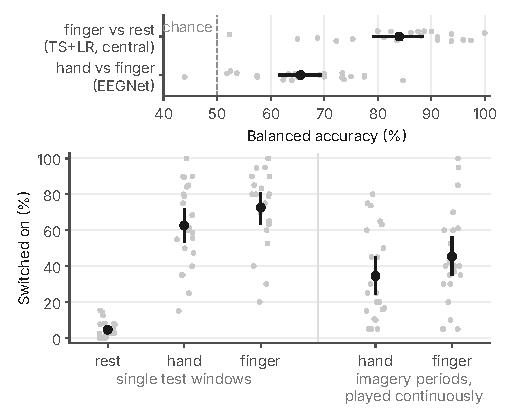
\includegraphics[width=0.9\linewidth]{paper_switch.pdf}
  \caption{The sixth finger used as a switch (exploratory, added after the results; runs 3--4,
  $n = \rqFourCueN$). Upper panels: TS+LR on the 14 central channels for sixth finger against
  rest, and the pre-trained, fine-tuned EEGNet for hand against sixth finger. Lower panels: the
  share of test windows of each type that switch it on, and the share of imagery periods that
  do so in the continuous replay. Grey: patients; black: mean with 95\,\% bootstrap CI. Hand
  imagery switches it on nearly as often as sixth-finger imagery.}
  \label{fig:switch}
  \end{minipage}\hfill
  \begin{minipage}[t]{0.485\textwidth}
  \vspace{0pt}\centering

  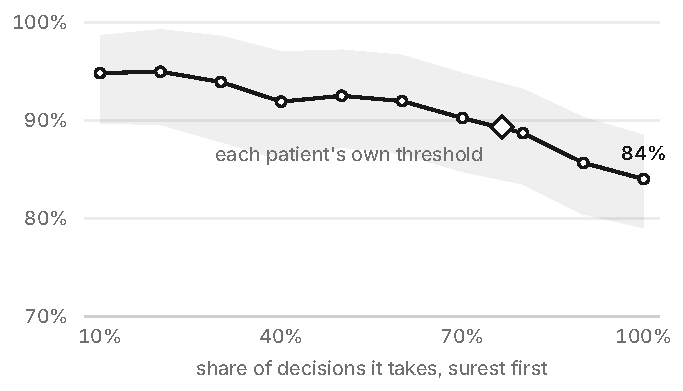
\includegraphics[width=0.9\linewidth]{web/switch-sure.pdf}
  \caption{Acting only when sure (exploratory). Accuracy of the central sixth-finger switch
  on the windows it acts on, against the share of windows it acts on, surest first; the band
  is a 95\,\% CI over patients, and the diamond marks the patients' own thresholds chosen on
  runs 1--2. Read from right to left: giving up the least certain decisions buys accuracy.}
  \label{fig:sure}
  \end{minipage}
\end{figure}

The gate costs the most. Replayed continuously, the sixth-finger switch caught
\exFiveFingerFingerOnMean\,\% of sixth-finger periods (CI
\exFiveFingerFingerOnCiLo--\exFiveFingerFingerOnCiHi) and \exFiveFingerHandOnMean\,\% of hand
periods, \exFiveFingerLatencyMean\,s after the cue of a 6\,s period, with
\exFiveFingerFalsePerMinMean{} false activations per minute of rest. A switch trained on rest
against any movement made fewer false activations than the demonstrator's network at a
similar detection rate, and a per-patient threshold on the gate changed neither clearly. The
three-class decoders of the pre-registered replay, whose gate looks for the sixth finger
itself, fared worst. No decoder drove the finger.
